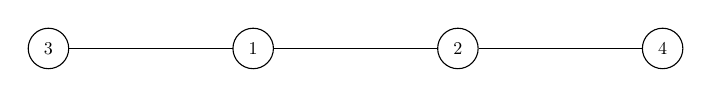
\begin{tikzpicture}[vertex/.style = {shape=circle,draw,minimum size=2.25em},scale=0.65, every node/.style={scale=0.65}]
    \node[vertex] (c1) at (-2,0) {$1$};
    \node[vertex] (c2) at (-6,0) {$3$};
    \node[vertex] (c3) at (2,0) {$2$};
    \node[vertex] (c4) at (6,0) {$4$};
    \draw (c1) -- (c2);
    \draw (c1) -- (c3);
    \draw (c3) -- (c4);
\end{tikzpicture}